\subsection{Correlation and Heatmap}

\begin{enumerate}
    \item Click on regression and select correlation from the drop down menu under classical.
    \item In the left panel, select the variables and move them to the Variables box.
    \item Check pearson’s correlation and heatmap.
\end{enumerate}

% Figure here-----------------------------
\begin{figure}[h]
\centering
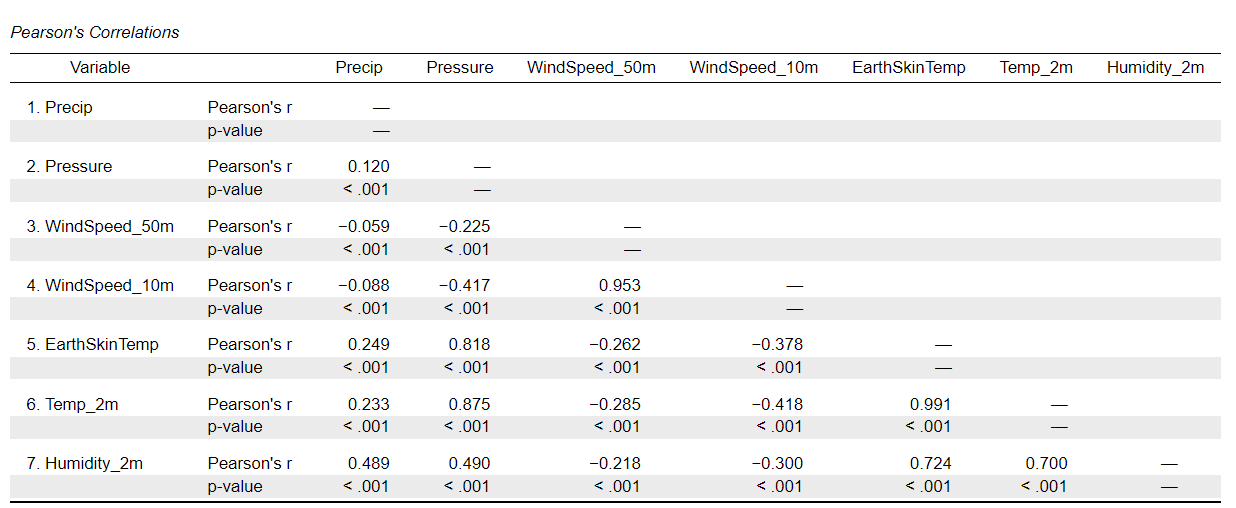
\includegraphics[width=0.7\textwidth]{figures/corr_jasp.png}
\caption{Pearson Correlation Matrix}
\end{figure}

% Figure here-----------------------------
\begin{figure}[h]
\centering
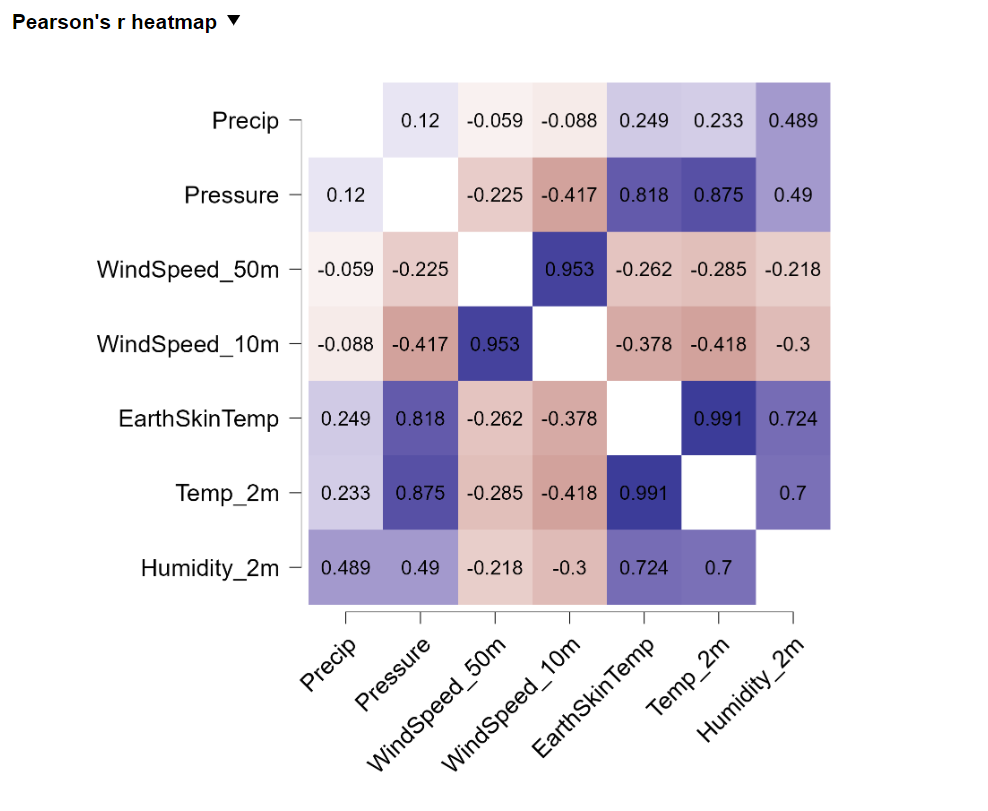
\includegraphics[width=0.7\textwidth]{figures/heatmap_jasp.png}
\caption{Heatmap}
\end{figure}

\clearpage